We test our stochastic trace estimator with both Chebyshev and Lanczos
approximation schemes on:
%
(1) a sound time series with missing data, using a GP with an RBF kernel;
%
(2) a three-dimensional space-time precipitation data set with over half a
million training points, using a GP with an RBF kernel; 
%
(3) a two-dimensional tree growth data set using a log-Gaussian Cox process
model with an RBF kernel;
%
(4) a three-dimensional space-time crime datasets with a log-Gaussian Cox model
with Mat\'ern 3/2 and spectral mixture kernels; and
%
(5) a high-dimensional feature space using the deep kernel learning framework 
\citep{wilson2016deep}. In the supplementary material we also include several
additional experiments to illustrate particular aspects of our approach,
including kernel hyperparameter recovery, diagonal corrections, and surrogate
methods. Throughout we use the SKI method \citep{wilson2015kernel} of Eq. 
\ref{eqn:ski} for fast MVMs. We find that the Lanczos and surrogate methods
are able to do kernel recovery and inference significantly faster and more
accurately than competing methods.

\subsection{Natural sound modeling}\label{sgpsec:sound}
Here we consider the natural sound benchmark in \cite{wilson2015kernel}, shown
in Figure \ref{fig:sound_data}. Our goal is to recover contiguous missing
regions in a waveform with $n = 59,306$ training points. We exploit Toeplitz
structure in the $\K{UU}$ matrix of our SKI approximate kernel for accelerated
MVMs.

The experiment in \cite{wilson2015kernel} only considered scalable inference and
prediction, but not hyperparameter learning, since the scaled eigenvalue
approach requires all the eigenvalues for an $m \times m$ Toeplitz matrix, which
can be computationally prohibitive with cost $\calO(m^2)$. However, evaluating
the marginal likelihood on this training set is not an obstacle for Lanczos and
Chebyshev since we can use fast MVMs with the SKI approximation at a cost of
$\calO(n + m \log m)$.

In Figure \ref{fig:sound_recovery}, we show how Lanczos, Chebyshev and
surrogate approaches scale with the number of inducing points $m$ compared to
the scaled eigenvalue method and FITC.  We use 5 probe vectors and 25 iterations
for Lanczos, both when building the surrogate and for hyperparameter learning
with Lanczos. We also use 5 probe vectors for Chebyshev and 100 moments. Figure 
\ref{fig:sound_recovery} shows the runtime of the hyperparameter learning phase
for different numbers of inducing points $m$, where Lanczos and the surrogate
are clearly more efficient than scaled eigenvalues and Chebyshev. For
hyperparameter learning, FITC took several hours to run, compared to minutes for
the alternatives; we therefore exclude FITC from Figure~
\ref{fig:sound_recovery}. Figure \ref{fig:sound_inference} shows the time to do
inference on the 691 test points,while \ref{fig:sound_smae} shows the
standardized mean absolute error (SMAE) on the same test points. As expected,
Lanczos and surrogate make accurate predictions much faster than Chebyshev,
scaled eigenvalues, and FITC.
%
In short, Lanczos and the surrogate approach are much faster than alternatives
for hyperparameter learning with a large number of inducing points and training
points.

\begin{figure}[ht]
  \begin{center}
    \begin{subfigure}{0.47\textwidth}
      \centering
      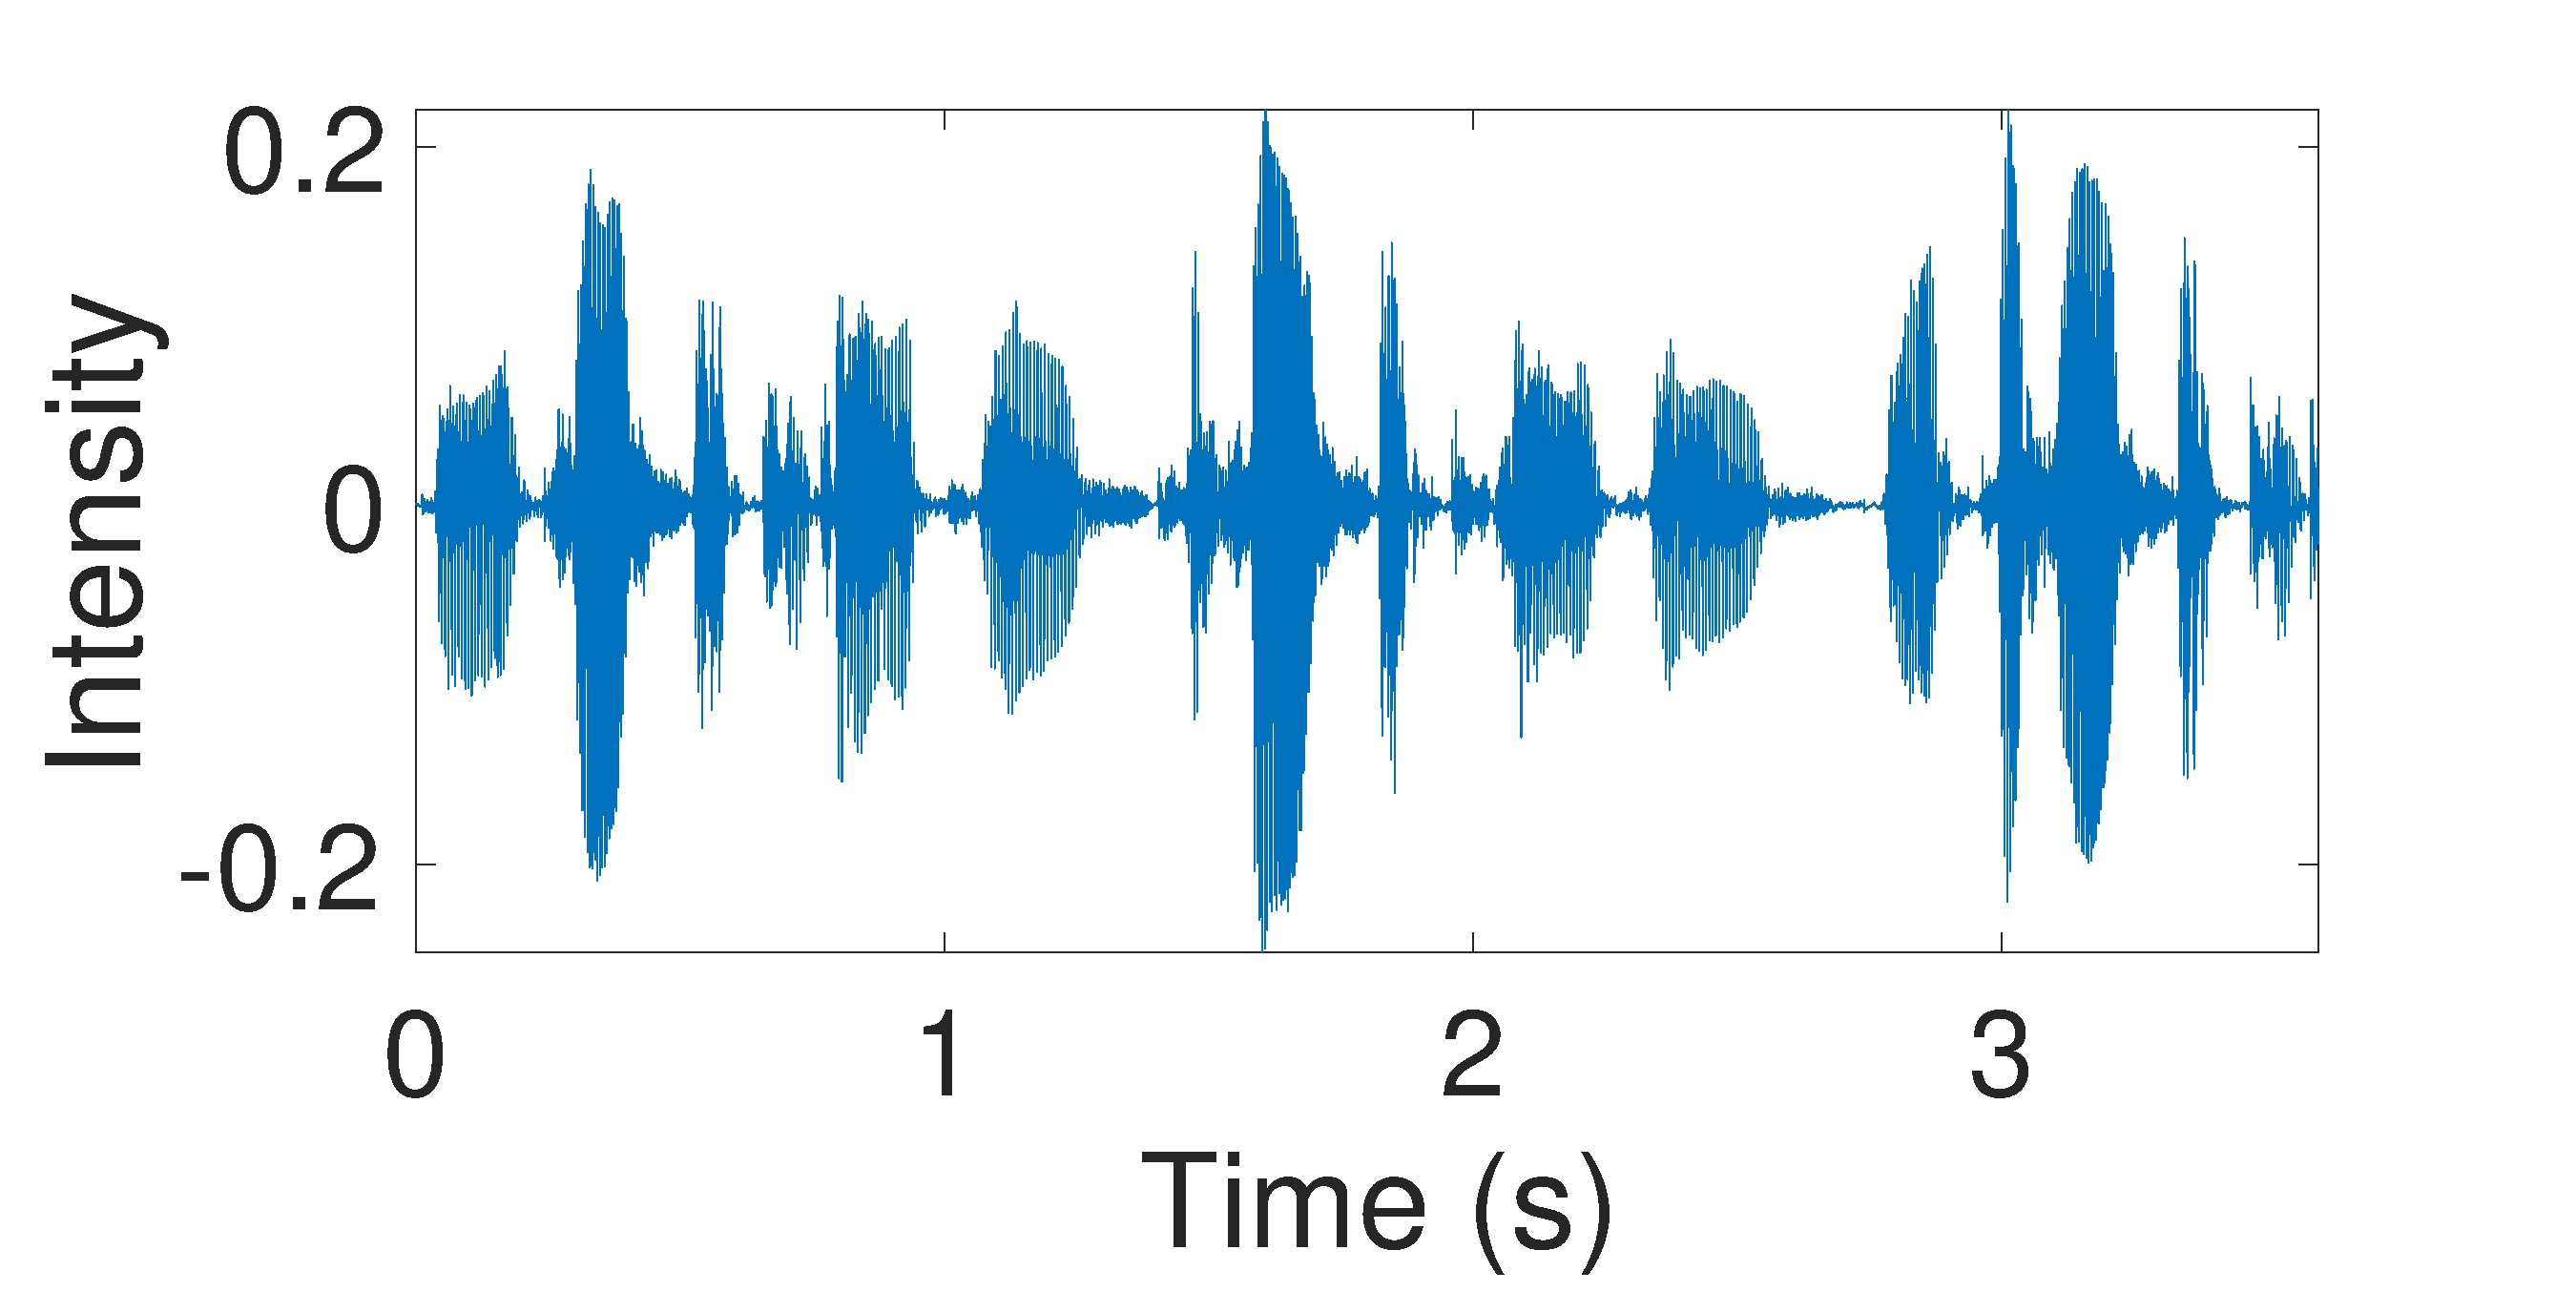
\includegraphics[width=\textwidth,trim=0.4cm 0cm 3.5cm 1.0cm,clip]
      {./sgp/pics/sound_data}
      \caption{Sound Data}
      \label{fig:sound_data}
    \end{subfigure}
    %
    \begin{subfigure}{0.47\textwidth}
      \centering
      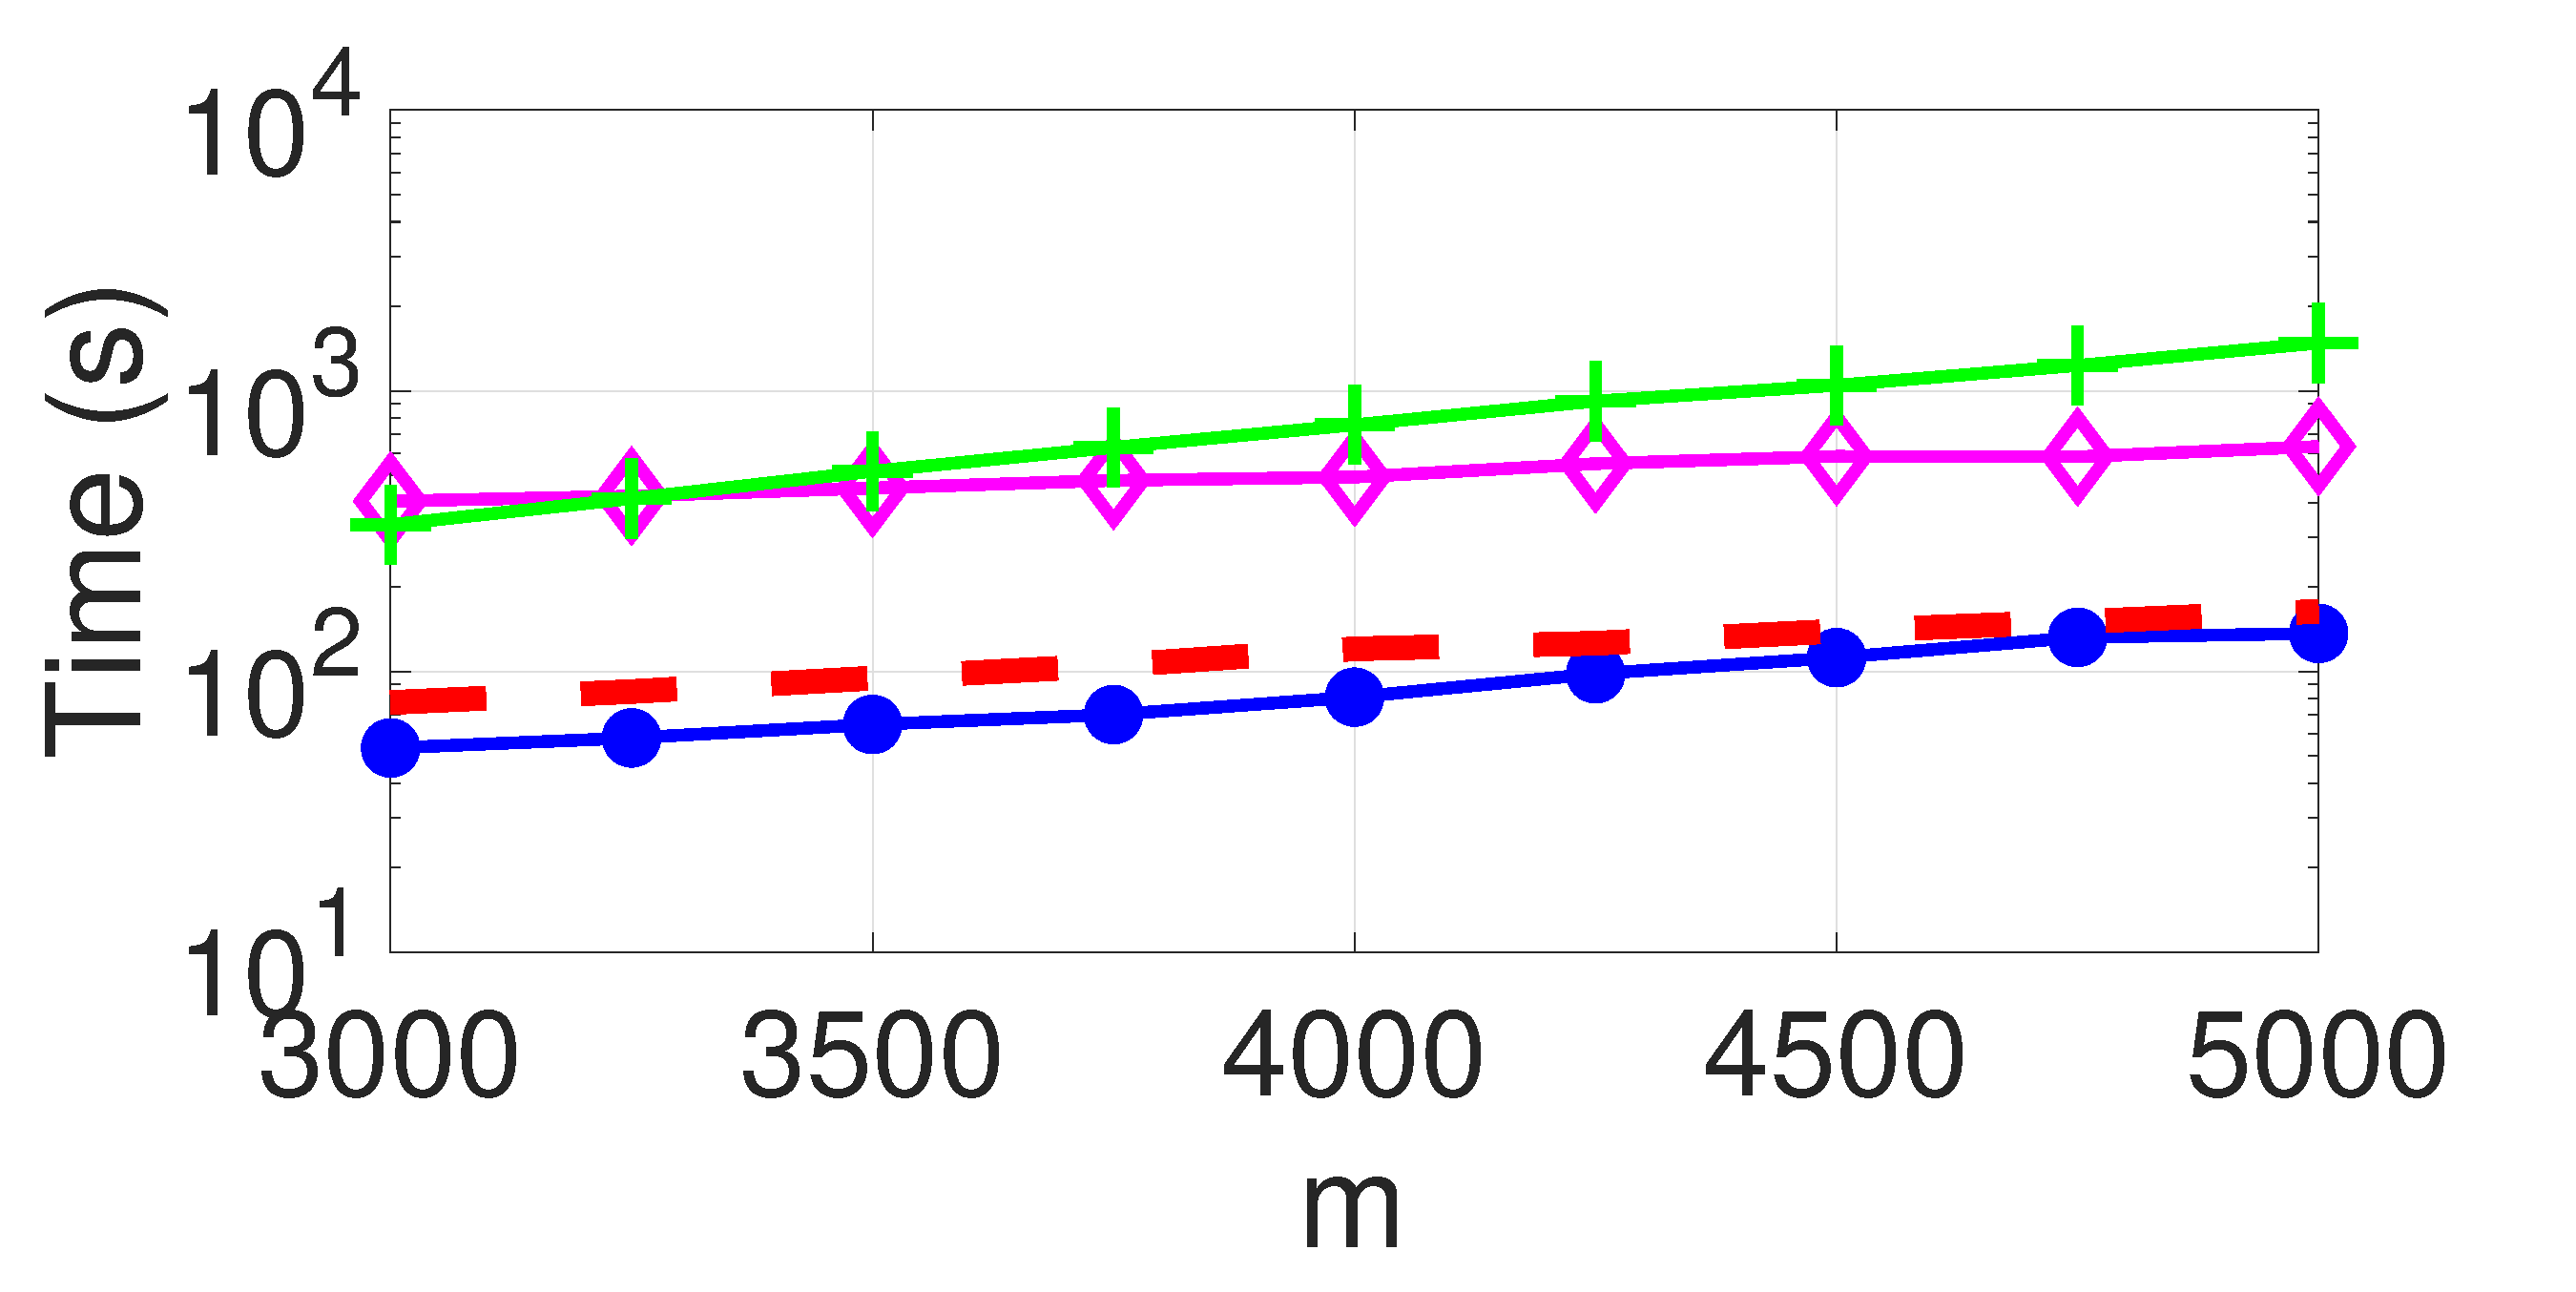
\includegraphics[width=\textwidth,trim=0.4cm 0cm 2.0cm 0cm,clip]
      {./sgp/pics/sound_recovery}
      \caption{Recovery Time}\label{fig:sound_recovery}
    \end{subfigure}
    %
    \begin{subfigure}{0.47\textwidth}
      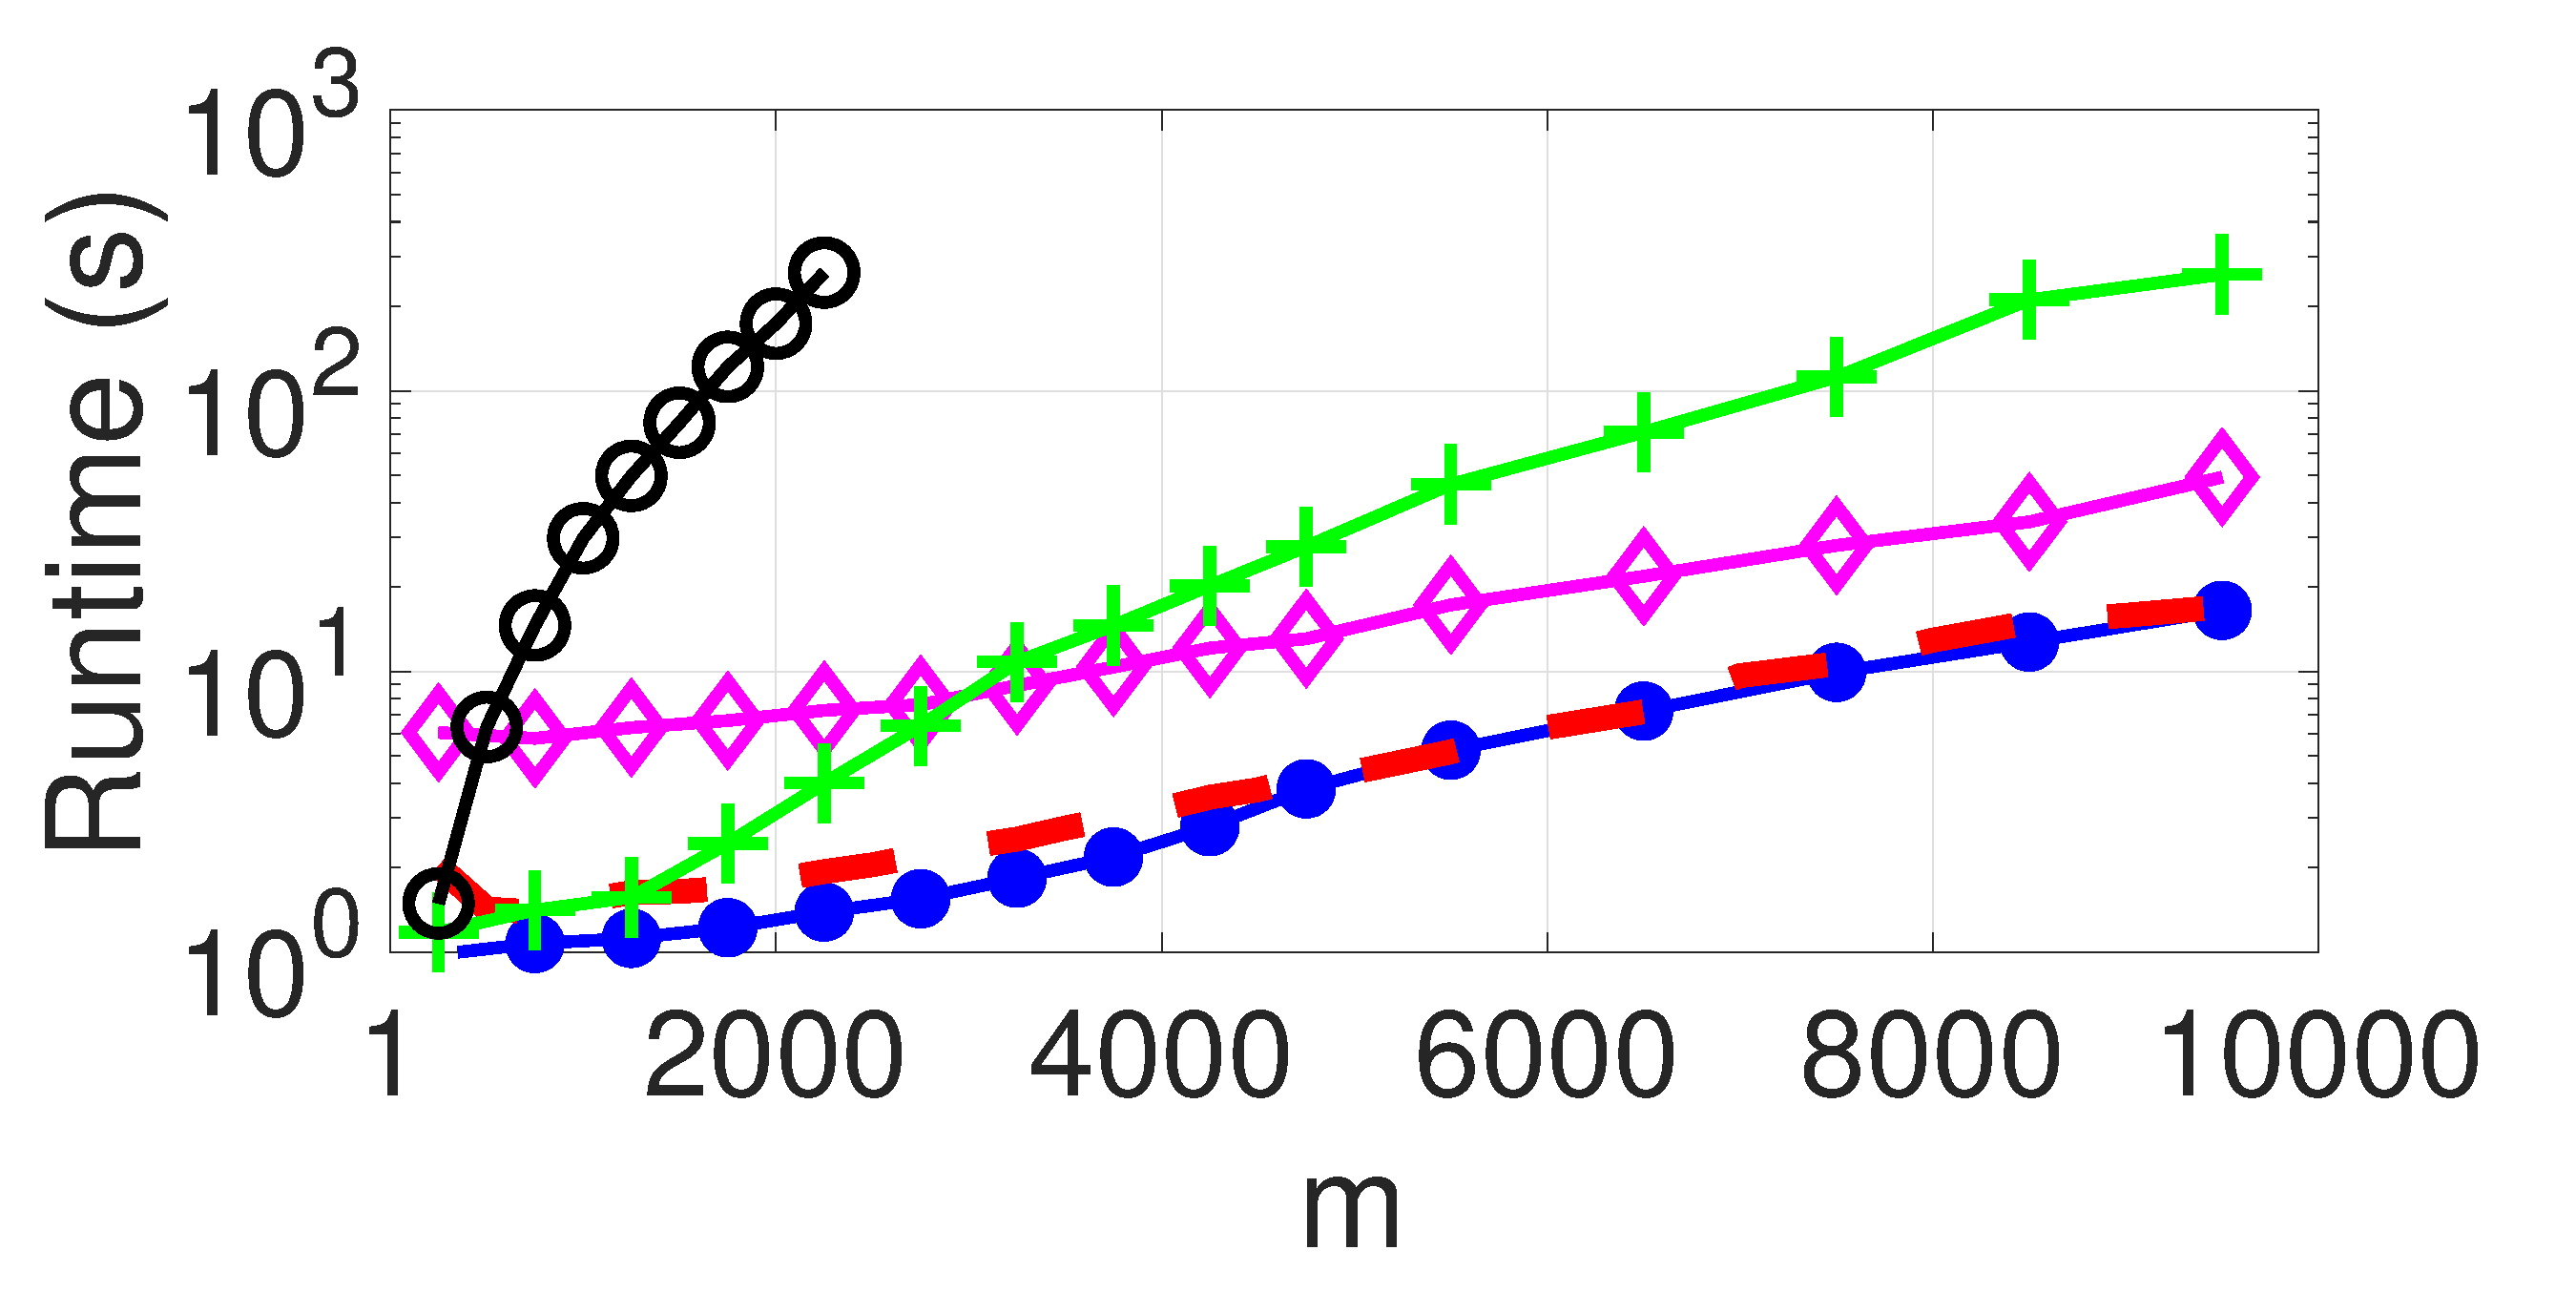
\includegraphics[width=\textwidth,trim=0.4cm 0cm 1.5cm 0.5cm,clip]
      {./sgp/pics/sound_inference}
      \caption{Inference Time}\label{fig:sound_inference}
    \end{subfigure}
    %
    \begin{subfigure}{0.47\textwidth}
      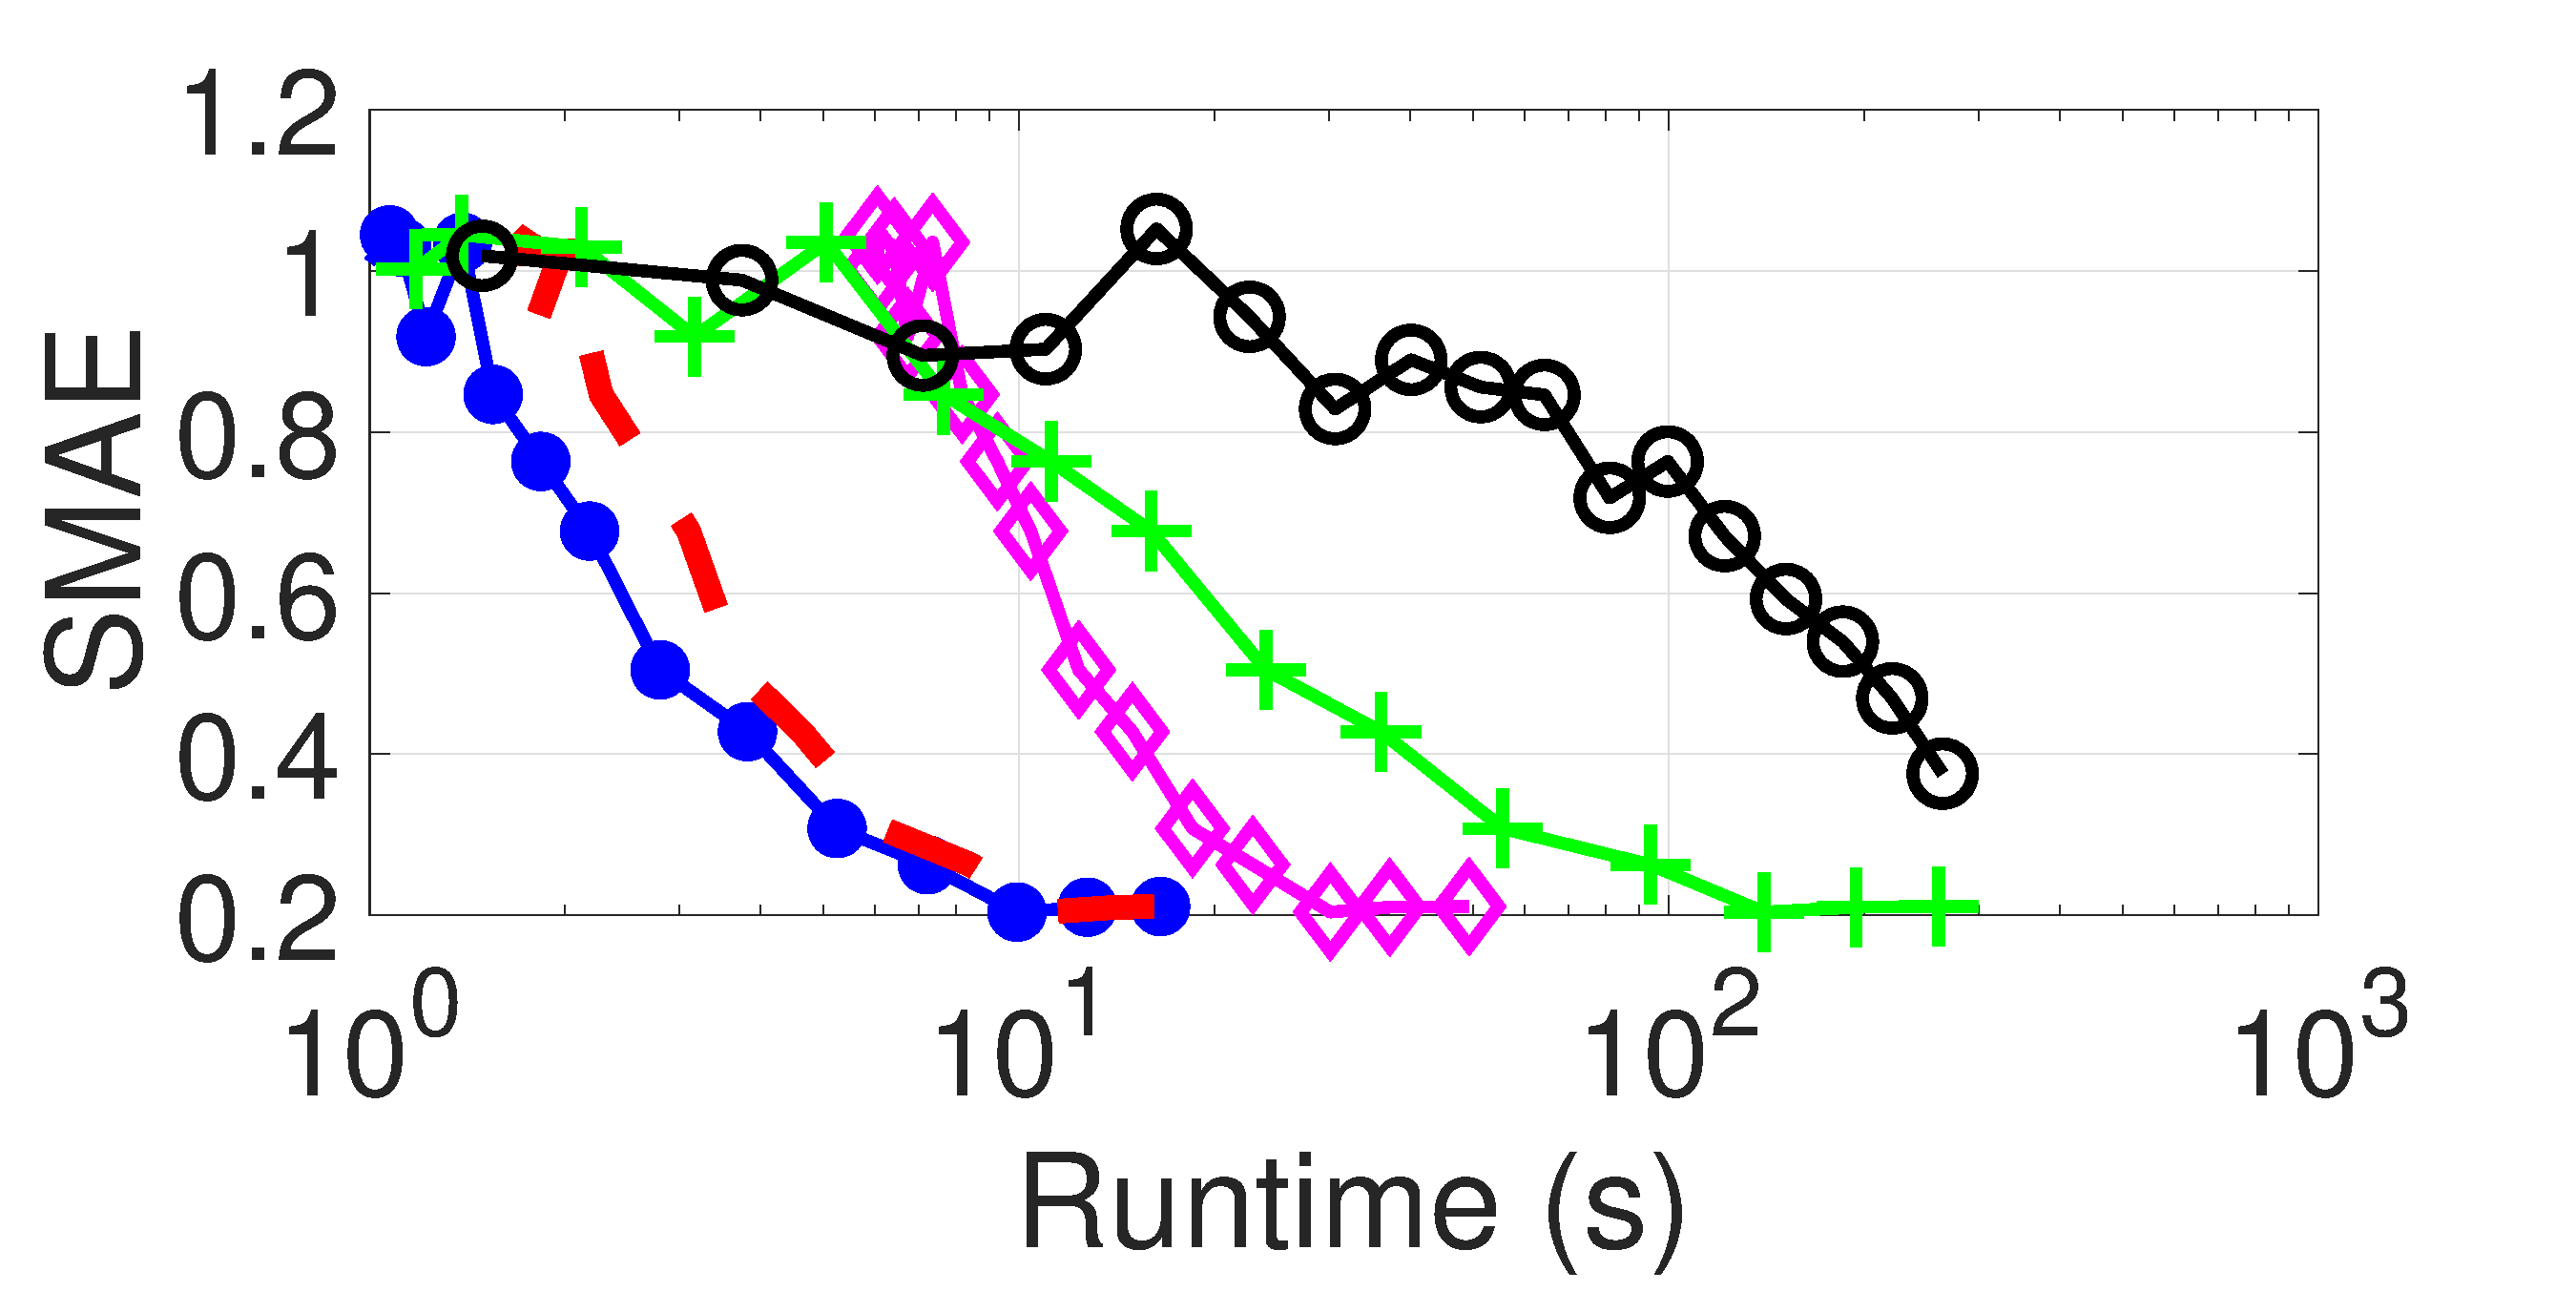
\includegraphics[width=\textwidth,trim=0.4cm 0cm 2.5cm 0.5cm,clip]
      {./sgp/pics/sound_smae}
      \caption{SMAE}\label{fig:sound_smae}
    \end{subfigure}
  \end{center}
  \caption{Sound modeling using 59,306 training points and 691 test points. The
  intensity of the time series can be seen in (a). Train time for RBF kernel
  hyperparameters is in (b) and the time for inference is in (c). The
  standardized mean absolute error (SMAE) as a function of time for an
  evaluation of the marginal likelihood and all derivatives is shown in (d).
  Surrogate is ({\color{blue} ------}), Lanczos is ({\color{red} - - -}),
  Chebyshev is {(\color{magenta} --- $\diamond$ ---}), scaled eigenvalues is ({
  \color{green} --- + ---}), and FITC is ({\color{black} --- o ---}).}
  \label{fig:sound_modeling}
\end{figure}

\subsection{Daily precipitation prediction}
This experiment involves precipitation data from the year of 2010 collected from
around $5500$ weather stations in the US\footnote{\url{https://catalog.data.gov/
dataset/u-s-hourly-precipitation-data}}. The hourly precipitation data is
preprocessed into daily data if full information of the day is available. The
dataset has $628,474$ entries in terms of precipitation per day given the date,
longitude and latitude. We randomly select $100,000$ data points as test points
and use the remaining points for training. We then perform hyperparameter
learning and prediction with the RBF kernel, using Lanczos, scaled eigenvalues,
and exact methods.

For Lanczos and scaled eigenvalues, we optimize the hyperparameters on the
subset of data for January 2010, with an induced grid of $100$ points per
spatial dimension and $300$ in the temporal dimension. Due to memory constraints
we only use a subset of $12,000$ entries for training with the exact method.
%
While scaled eigenvalues can perform well when fast eigendecompositions are
possible, as in this experiment, Lanczos nonetheless still runs faster and with
slightly lower mean square error (MSE).

\begin{table}[ht]
  \centering
  \caption{Prediction Comparison for the Daily Precipitation Data
  \textsuperscript{$\alpha$}.}\label{tab:precip}
  \begin{threeparttable}
    \begin{tabular}{r c c c c}
      \toprule
      Method  & \#Training Pts   & \#Induced Pts & MSE & Time [min]\\ \midrule
      Lanczos & 528k  & 3M  & 0.613 &  14.3\\
      Scaled\hyp{}Eig & 528k  & 3M  & 0.621 &  15.9\\
      Exact   & 12k   & -   & 0.903 &  11.8\\
      \bottomrule
    \end{tabular}
    \begin{tablenotes}
      \item[$\alpha$] The columns are the number of training points, number of
      induced grid points, mean squared error, and inference time.
    \end{tablenotes}
  \end{threeparttable}
\end{table}
Incidentally, we are able to use 3 \emph{million} inducing points in Lanczos and
scaled eigenvalues, which is enabled by the SKI representation 
\citep{wilson2015kernel} of covariance matrices, for a a very accurate
approximation.  This number of inducing points $m$ is unprecedented for typical
alternatives which scale as $\calO(m^3)$.


\subsection{Hickory data}
In this experiment, we apply Lanczos to the log-Gaussian Cox process model with
a Laplace approximation for the posterior distribution. We use the RBF kernel
and the Poisson likelihood in our model.  The scaled eigenvalue method does not
apply directly to non-Gaussian likelihoods; we thus applied the scaled
eigenvalue method in \citep{wilson2015kernel} in conjunction with the Fiedler
bound in \citep{flaxman2015fast} for the scaled eigenvalue comparison.  Indeed,
a key advantage of the Lanczos approach is that it can be applied whenever fast
MVMs are available, which means no additional approximations such as the Fiedler
bound are required for non-Gaussian likelihoods.

This dataset, which comes from the R package {\tt spatstat}, is a point pattern
of $703$ hickory trees in a forest in Michigan. We discretize the area into a
$60 \times 60$ grid and fit our model with exact, scaled eigenvalues, and
Lanczos. We see in Table \ref{tab:hickory} that Lanczos recovers hyperparameters
that are much closer to the exact values than the scaled eigenvalue approach.
Figure \ref{fig:hickory} shows that the predictions by Lanczos are also
indistinguishable from the exact computation.

\begin{table}[ht]
  \centering
  \caption{Hyperparameters Recovered on the Hickory Dataset.}\label{tab:hickory}
  \begin{tabular}{r c c c c c}
    \toprule
    Method & $s_f$ & $\ell_1$ & $\ell_2$ & $-\log p(y|\theta)$ & Time [s]\\
    \midrule
    Exact & $0.696$  & $0.063$  & $0.085$ &  $1827.56$ & $465.9$\\
    Lanczos & $0.693$   & $0.066$   & $0.096$ &  $1828.07$ & $21.4$\\
    Scaled\hyp{}Eig & $0.543$  & $0.237$  & $0.112$ &  $1851.69$ & $2.5$\\
    \bottomrule
  \end{tabular}
\end{table}
\vfill

\begin{figure}[ht]
  \begin{center}
    \begin{subfigure}{0.3\textwidth}
      \centering
      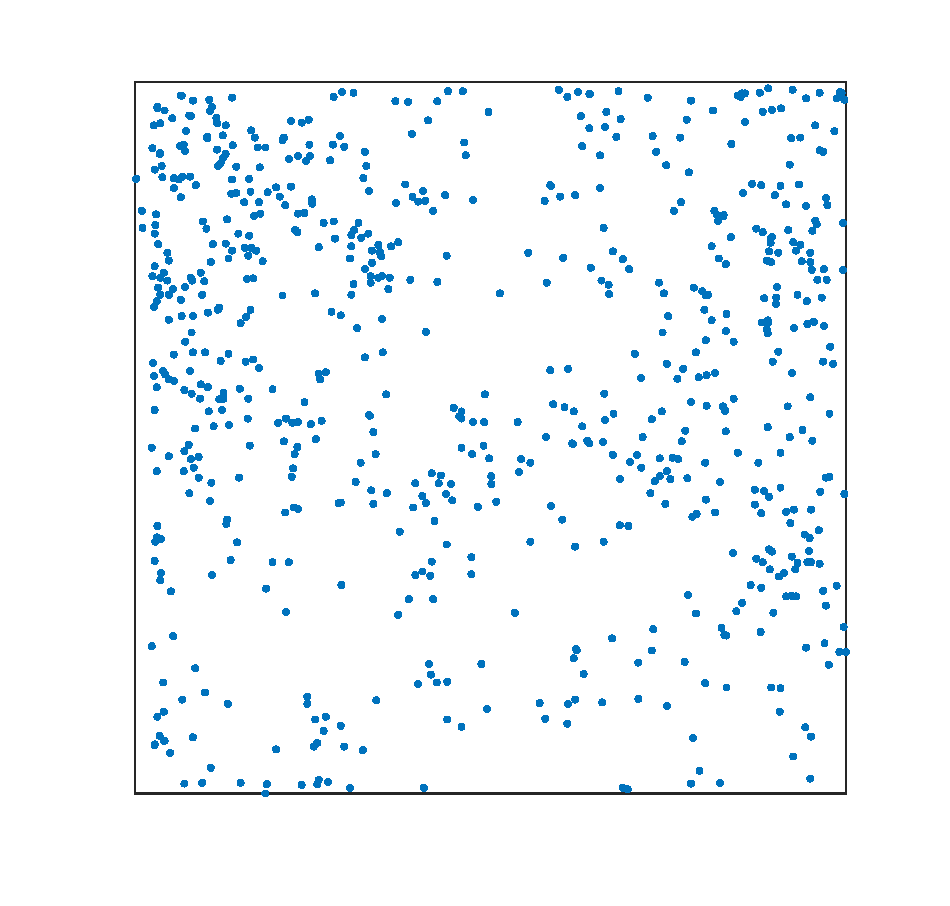
\includegraphics[height=0.87\textwidth,trim = 1cm 1cm 1cm 1cm,clip]
      {./sgp/pics/Hickory_point.eps}
      \caption{Point Pattern Data}\label{fig:hpoint}
    \end{subfigure}
    \hspace{1cm}
    \begin{subfigure}{0.3\textwidth}
      \centering
      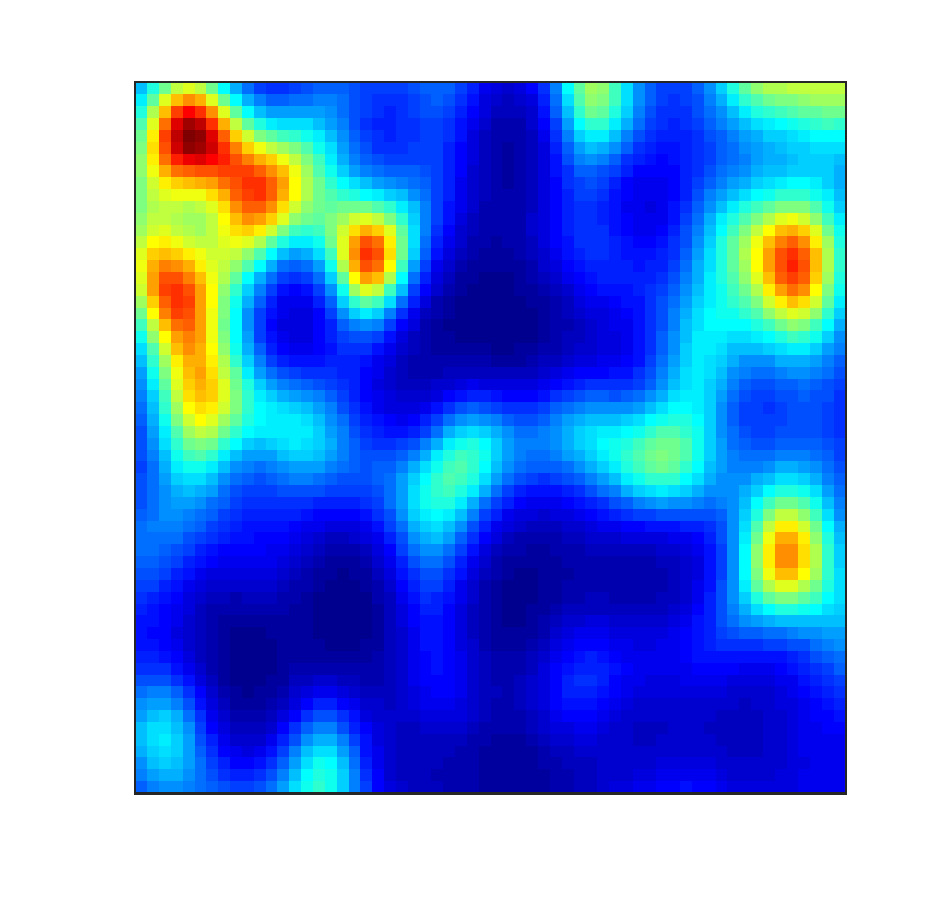
\includegraphics[height=0.87\textwidth,trim = 1cm 1cm 1cm 1cm,clip]
      {./sgp/pics/Hickory_exact.eps}
      \caption{Prediction by Exact}\label{fig:hickory_exact}
    \end{subfigure}
    \linebreak
    \begin{subfigure}{0.3\textwidth}
      \centering
      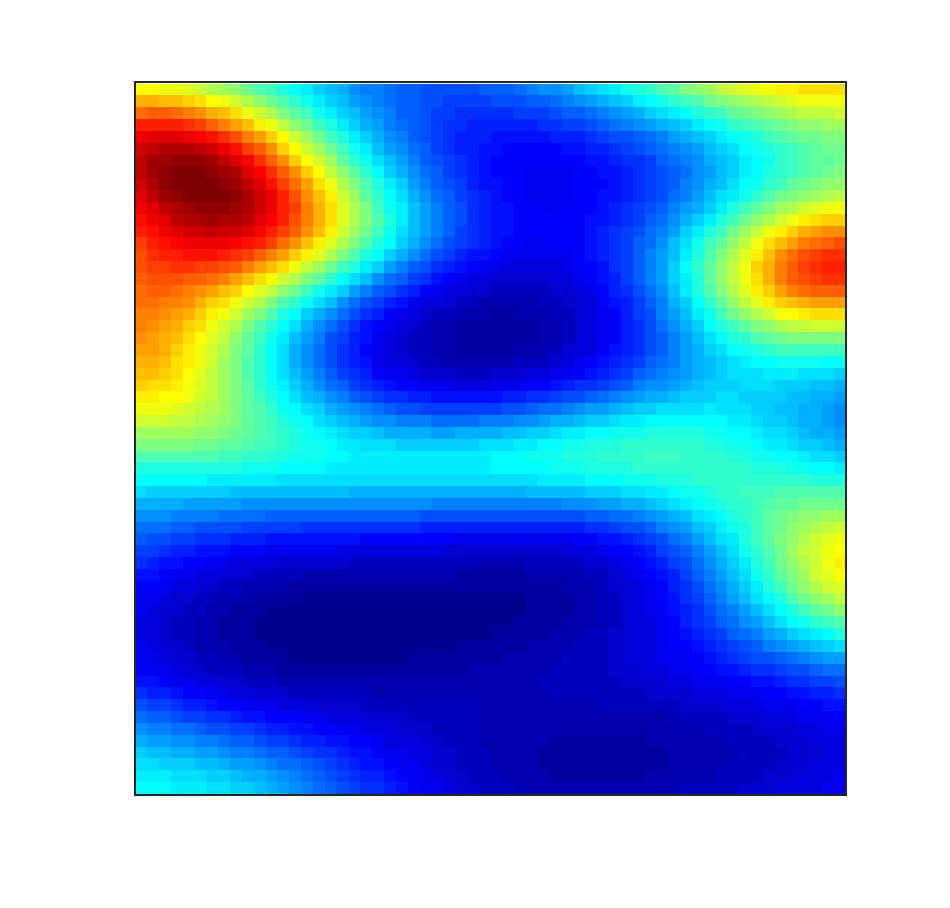
\includegraphics[height=0.87\textwidth,trim = 1cm 1cm 1cm 1cm,clip]
      {./sgp/pics/Hickory_ski.eps}
      \caption{Scaled\hyp{}Eig}\label{fig:hickory_ski}
    \end{subfigure}
    \hspace{1cm}
    \begin{subfigure}{0.3\textwidth}
      \centering
      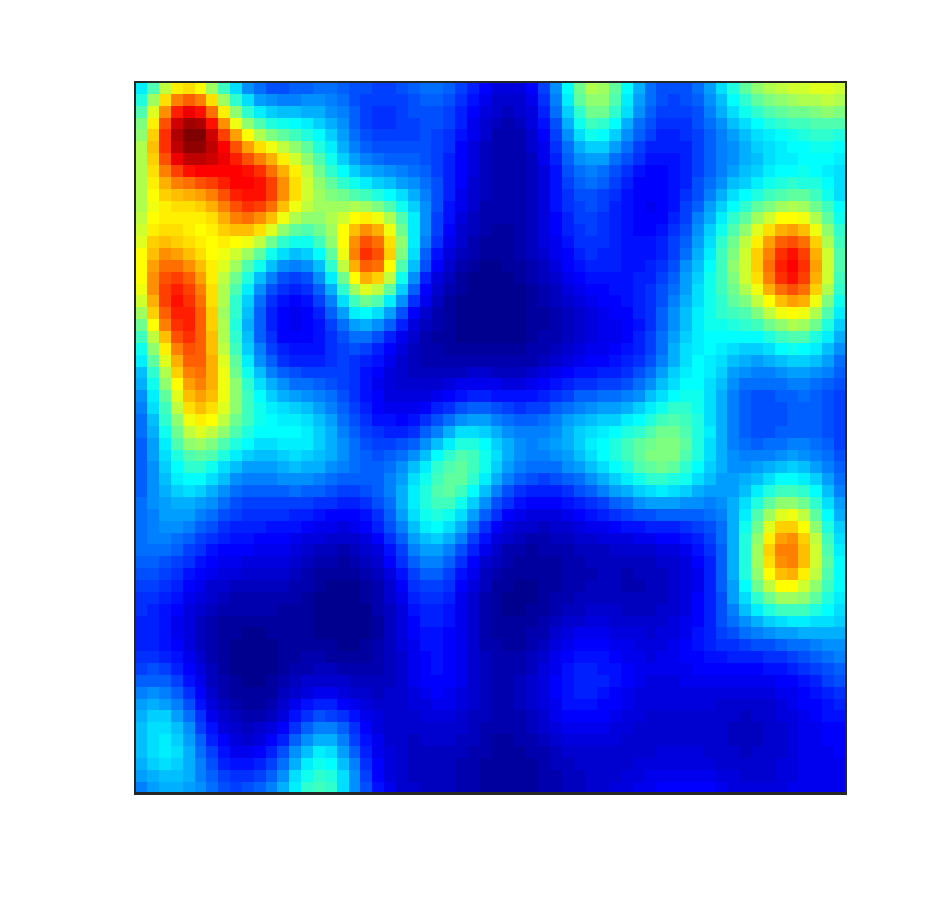
\includegraphics[height=0.87\textwidth,trim = 1cm 1cm 1cm 1cm,clip]
      {./sgp/pics/Hickory_lan.eps}
      \caption{Lanczos}\label{fig:hickory_lan}
    \end{subfigure}
    \caption{Predictions by exact, scaled eigenvalues, and Lanczos on the Hickory dataset.}\label{fig:hickory}
  \end{center}
\end{figure}

\subsection{Crime prediction}
In this experiment, we apply Lanczos with the spectral mixture kernel to the
crime forecasting problem considered in \cite{flaxman2015fast}. This dataset
consists of $233,088$ incidents of assault in Chicago from January 1, 2004 to
December 31, 2013. We use the first $8$ years for training and attempt to
predict the crime rate for the last $2$ years. For the spatial dimensions, we
use the log-Gaussian Cox process model, with the Mat\'ern-5/2 kernel, the
negative binomial likelihood, and the Laplace approximation for the posterior.
We use a spectral mixture kernel with $20$ components and an extra constant
component for the temporal dimension. We discretize the data into a $17 \times
26$ spatial grid corresponding to $1\mile\Times1\mile$ grid cells. In
the temporal
dimension we sum our data by weeks for a total of $522$ weeks. After removing
the cells that are outside Chicago, we have a total of $157,644$ observations.

The results for Lanczos and scaled eigenvalues (in conjunction with the Fiedler
bound due to the non-Gaussian likelihood) can be seen in Table 
\ref{tab:chicago_homicide}. The Lanczos method used $5$ Hutchinson probe vectors
and $30$ Lanczos steps. For both methods we allow $100$ iterations of LBFGS to
recover hyperparameters and we often observe early convergence. While the root
mean square error (RMSE) for Lanczos and scaled eigenvalues happen to be close
on this example, the recovered hyperparameters using scaled eigenvalues are very
different than for Lanczos. For example, the scaled eigenvalue method learns
much larger $\sigma^2$ than Lanczos, indicating model misspecification. In
general, as the data become increasingly non-Gaussian the Fiedler bound (used
for fast scaled eigenvalues on non-Gaussian likelihoods) will become
increasingly misspecified, while Lanczos will be unaffected.

\begin{table}[ht]
  \centering
  \caption{Hyperparameters Recovered, Recovery Time and RMSE for Lanczos and
  Scaled Eigenvalues on the Chicago Assault Data\textsuperscript{$\alpha$}.}
  \label{tab:chicago_homicide}
  \begin{threeparttable}
    \begin{tabular}{r c c c c c c c}
      \toprule
      Method & $\ell_1$ & $\ell_2$ & $\sigma^2$ & T\textsubscript{recovery}[s]&
      T\textsubscript{prediction}[s] & RMSE\textsubscript{train} &
      RMSE\textsubscript{test} \\
      \midrule
      Lanczos & 0.65 & 0.67 & \ph69.72 & 264 & 10.30 & 1.17 & 1.33 \\
      Scaled\hyp{}Eig & 0.32 & 0.10 & 191.17 & \ph67 & \ph3.75 & 1.19 & 1.36 \\
      \bottomrule
    \end{tabular}
    \begin{tablenotes}
      \item[$\alpha$] $\ell_1$ and $\ell_2$ are the length scales in
      spatial dimensions. $\sigma^2$ is the noise level.
      T\textsubscript{recovery} is the time for recovering hyperparameters.
      T\textsubscript{prediction} is the time for prediction at all $157,644$
      observations, including training and testing.
    \end{tablenotes}
  \end{threeparttable} 
\end{table}

\subsection{Deep kernel learning}
To handle high-dimensional datasets, we bring our methods into the deep kernel
learning framework \cite{wilson2016deep} by replacing the final layer of a
pre-trained deep neural network (DNN) with a GP. This experiment uses the gas
sensor dataset from the UCI machine learning repository. It has $2565$ instances
with $128$ dimensions. We pre-train a DNN, then attach a Gaussian process with
RBF kernels to the two-dimensional output of the second-to-last layer. We then
further train all parameters of the resulting kernel, \emph{including} the
weights of the DNN, through the GP marginal likelihood. In this example, Lanczos
and the scaled eigenvalue approach perform similarly well.  Nonetheless, we see
that Lanczos can effectively be used with SKI on a high dimensional problem to
train hundreds of thousands of kernel parameters.

\vfill
\begin{table}[ht]
  \centering
  \caption{Prediction RMSE and Per Training Iteration Runtime.}\label{tab:dkl}
  \begin{tabular}{r c c c}
    \toprule
    Method & DNN & Lanczos & Scaled\hyp{}Eig \\
    \midrule
    RMSE & $0.1366\pm 0.0387$ & $0.1053\pm0.0248$ & $0.1045\pm 0.0228$\\
    Time [s]& $0.4438$ & $2.0680$ & $1.6320$\\
    \bottomrule
  \end{tabular} 
\end{table}
\vfill